\documentclass[10pt,twocolumn]{article}

% Line spacing
\renewcommand{\baselinestretch}{1.05}
\widowpenalty=10000
\clubpenalty=10000
\hyphenpenalty=300
\tolerance=1000

% Packages
\usepackage[T1]{fontenc}
\usepackage{mathpazo}
\usepackage[scaled=0.9]{helvet}
\usepackage{courier}
\usepackage{microtype}
\usepackage{graphicx}
\usepackage{amsmath}
\usepackage{amssymb}
\usepackage{booktabs}
\usepackage{tabularx}
\usepackage{xcolor}
\usepackage{listings}
\PassOptionsToPackage{hyphens,spaces,obeyspaces}{url}
\usepackage[round,authoryear]{natbib}
\bibliographystyle{plainnat}
\usepackage{hyperref}
\usepackage{cleveref}
\usepackage{enumitem}
\usepackage{titlesec}
\usepackage{subcaption}
\usepackage{svg}

% Caption styling
\usepackage{caption}
\captionsetup{font=small, labelfont=bf, labelsep=period, justification=justified, singlelinecheck=false, skip=8pt}
\captionsetup[table]{position=top}

% Section spacing
\titlespacing*{\section}{0pt}{0.8\baselineskip}{0.5\baselineskip}
\titlespacing*{\subsection}{0pt}{0.6\baselineskip}{0.4\baselineskip}
\titlespacing*{\subsubsection}{0pt}{0.5\baselineskip}{0.3\baselineskip}

% Page geometry
\usepackage[letterpaper, top=0.75in, bottom=1in, left=0.65in, right=0.65in]{geometry}

% Colors
\definecolor{harvardcrimson}{HTML}{A31F34}
\definecolor{codegreen}{HTML}{2D7A2D}
\definecolor{codegray}{HTML}{555555}
\definecolor{lightgray}{HTML}{F5F5F5}

% Hyperref setup
\hypersetup{
  colorlinks=true,
  linkcolor=harvardcrimson,
  citecolor=harvardcrimson,
  urlcolor=harvardcrimson
}

% Code listing style
\lstset{
  basicstyle=\ttfamily\small,
  backgroundcolor=\color{lightgray},
  frame=single,
  rulecolor=\color{codegray},
  breaklines=true,
  showstringspaces=false
}

% Custom commands — updated to reflect the new system
\newcommand{\staffml}{\textsc{StaffML}}
\newcommand{\numquestions}{5{,}786}
\newcommand{\numpublished}{5{,}786}
\newcommand{\numtracks}{5}
\newcommand{\numlevels}{6}
\newcommand{\numtopics}{79}
\newcommand{\numareas}{13}
\newcommand{\numzones}{11}
\newcommand{\numedges}{123}
\newcommand{\numchains}{1{,}011}
\newcommand{\numfullchains}{177}
\newcommand{\numinvariants}{19}

% ============================================================================
\begin{document}

\title{
  \textbf{StaffML: A Physics-Grounded Interview Question Bank\\
  for Machine Learning Systems Engineers}\\[0.3em]
  {\large System Design, Competency Model, and Quality Infrastructure}
}

\author{
  Vijay Janapa Reddi\\
  Harvard University\\
  \texttt{vj@eecs.harvard.edu}
}

\date{Working Draft --- \today}

\maketitle

% ============================================================================
\begin{abstract}
We present \staffml{}, a curated bank of \numquestions{} interview questions for ML systems engineers spanning \numtracks{} deployment tracks (cloud, edge, mobile, TinyML, global) and \numlevels{} mastery levels mapped to Bloom's revised taxonomy. Every question is classified on four independent axes: \emph{topic} (79 curated concepts organized into 13 competency areas with a prerequisite graph), \emph{zone} (11 ikigai-inspired cognitive zones that capture \emph{how} a topic is tested), \emph{track} (which physics regime the question targets), and \emph{level} (what cognitive depth is required).

Unlike existing interview preparation resources that focus on algorithmic coding, \staffml{} tests \emph{mechanical sympathy}---the ability to reason quantitatively about the physical constraints of ML infrastructure. Every question requires napkin math grounded in real hardware specifications: memory bandwidth limits, thermal envelopes, interconnect topologies, and the economics of accelerator fleets.

The key intellectual contribution is the \emph{ikigai competency model}: four fundamental skills---recall, analyze, design, implement---whose pairwise intersections produce six compound cognitive zones (diagnosis, specification, fluency, evaluation, realization, optimization) and whose union yields a mastery zone. This model replaces traditional flat taxonomies with a structured vocabulary for what it means to ``know'' ML systems engineering. The classification schema is defined in LinkML and generates Pydantic models, JSON Schema, and TypeScript types from a single source of truth. Quality is enforced by a 19-check invariant system, multi-model math verification, and three-stage deduplication.
\end{abstract}

% ============================================================================
\section{Introduction}
\label{sec:intro}

The role of the ML systems engineer has emerged as one of the most sought-after positions in the technology industry. Unlike ML researchers who design model architectures or software engineers who write application code, ML systems engineers must reason about the \emph{physical constraints} of deploying machine learning at scale: memory bandwidth limits that determine whether a workload is compute-bound or memory-bound, thermal envelopes that cap sustained throughput on edge devices, network congestion that dominates training time in distributed clusters, and the economics of accelerator fleets where a single misconfigured batch size can waste thousands of dollars per hour.

Yet interview preparation resources for this role are remarkably thin. LeetCode \citep{leetcode2024} offers 2,800+ algorithmic coding problems but nothing on GPU memory hierarchies or KV-cache sizing. Chip Huyen's \emph{Designing Machine Learning Systems} \citep{huyen2022designing} provides excellent conceptual coverage but no interactive, quantitative practice. Mock interview platforms like Interviewing.io focus on behavioral and coding rounds, not system design with napkin math. The result is a preparation gap: candidates study the wrong material, and interviewers lack a validated question bank calibrated to the specific cognitive demands of systems reasoning.

\staffml{} fills this gap with \numquestions{} questions that test \emph{mechanical sympathy}---the term originally coined by Martin Thompson for software that works \emph{with} the hardware rather than against it. Every question has:

\begin{itemize}[nosep]
  \item A realistic interview \textbf{scenario} drawn from industry practice
  \item A \textbf{common mistake} that candidates typically make
  \item A \textbf{realistic solution} with quantitative reasoning
  \item \textbf{Napkin math} grounded in real hardware specifications
  \item Classification by \textbf{topic} (what concept), \textbf{zone} (how it is tested), \textbf{track} (where it deploys), and \textbf{level} (how hard it is)
\end{itemize}

\staffml{} is the companion assessment tool for the \emph{Machine Learning Systems} textbook \citep{reddi2026mlsys}, developed alongside the Harvard CS249r course \citep{cs249r}. The textbook teaches quantitative reasoning about ML infrastructure---memory hierarchies, parallelism strategies, serving architectures---and \staffml{} provides the practice that reinforces that reasoning. Questions reference the same hardware constants, use the same ``constraints drive architecture'' philosophy, and map to the same deployment tracks (cloud, edge, mobile, TinyML) covered in the two-volume curriculum.

This paper is organized as follows. \Cref{sec:motivation} establishes the first-principles motivation for a physics-grounded approach to ML systems interview preparation. \Cref{sec:competency-model} presents the ikigai competency model---the intellectual centerpiece of the classification system. \Cref{sec:topics} describes the 79-topic taxonomy with its prerequisite graph. \Cref{sec:tracks} explains the physics-based rationale for the five deployment tracks. \Cref{sec:examples} presents example questions at different cognitive zones. \Cref{sec:qa} covers the multi-stage quality assurance process. \Cref{sec:coverage} analyzes corpus coverage. \Cref{sec:infrastructure} describes the vault toolchain and schema infrastructure. \Cref{sec:status} reports current status and future work.

\begin{table}[t]
\centering
\small
\caption{\staffml{} vault summary statistics.}
\label{tab:summary}
\begin{tabular}{@{}lr@{}}
\toprule
\textbf{Metric} & \textbf{Value} \\
\midrule
Published questions & \numpublished{} \\
Deployment tracks & \numtracks{} \\
Mastery levels (Bloom's) & \numlevels{} \\
Curated topics & \numtopics{} \\
Competency areas & \numareas{} \\
Ikigai zones & \numzones{} \\
Prerequisite graph edges & \numedges{} \\
Depth chains ($\geq 3$ levels) & \numchains{} \\
Full chains (L1$\to$L6+) & \numfullchains{} \\
Invariant checks & \numinvariants{} \\
Napkin math coverage & 100\% \\
Schema definition & LinkML \\
\bottomrule
\end{tabular}
\end{table}

% ============================================================================
\section{Why ML Systems Interview Preparation}
\label{sec:motivation}

\subsection{A Distinct Engineering Discipline}

The ML systems engineer occupies a unique position at the intersection of three disciplines---yet belongs fully to none of them. An ML \emph{researcher} designs model architectures and loss functions but may never consider whether the model fits in HBM or how attention scales with sequence length on real silicon. A \emph{software engineer} writes reliable, tested code but may never reason about memory bandwidth, arithmetic intensity, or the roofline model. The ML systems engineer must do both, and more: they must reason about the \emph{physical constraints} that govern how models execute on real hardware.

This is what Martin Thompson calls \emph{mechanical sympathy}---the principle that software performs best when developers understand the hardware it runs on. A Formula 1 driver who understands the engine does not merely drive faster; they drive \emph{differently}, making decisions that are physically impossible to arrive at through pure algorithmic thinking. Similarly, an ML systems engineer who understands that HBM3 access is $\sim$300$\times$ slower than an L1 register read does not merely optimize code---they \emph{architect} systems that minimize data movement in the first place.

\subsection{Constraints Drive Architecture}

The intellectual foundation of \staffml{} is the thesis that \textbf{constraints drive architecture}. You do not choose a Transformer because it is trendy; you choose it because its attention mechanism parallelizes across thousands of cores on real silicon, unlike the sequential dependency chains of RNNs. You do not use mixed precision because a tutorial told you to; you use it because FP16 tensor cores deliver $2\times$ the throughput of FP32 and halve the memory footprint, changing whether your model fits on one GPU or requires four.

This philosophy, drawn from the \emph{Machine Learning Systems} textbook \citep{reddi2026mlsys}, insists that AI is not magic---it is infrastructure, and infrastructure has laws. These laws are rooted in physics: the speed of light bounds interconnect latency, thermodynamics caps sustained power draw, and Shannon's theorem limits how much information a wire can carry. A Staff+ engineer who internalizes these constraints can \emph{derive} optimal architectures from first principles rather than memorizing best practices that may be obsolete by next year.

\subsection{Why Existing Preparation Fails}

Existing interview preparation platforms fail ML systems candidates in three specific ways:

\textbf{LeetCode tests algorithms, not systems.} A candidate who can implement Dijkstra's algorithm in $O(E \log V)$ may not know that the same GPU running inference at batch size 1 is $50\times$ less efficient than at batch size 32---because the workload shifts from memory-bound to compute-bound past the roofline ridge point. LeetCode's 2,800+ problems develop important skills, but none of them test whether a candidate can size a KV-cache, estimate serving throughput, or diagnose why GPU utilization dropped from 80\% to 4\%.

\textbf{Conceptual resources lack quantitative practice.} Chip Huyen's textbook \citep{huyen2022designing} teaches what a feature store is, what data drift means, and how to think about ML system design. But it does not ask the candidate to \emph{calculate} how many tokens per second an H100 can generate for a 70B model, or \emph{derive} the memory bandwidth required to sustain that throughput. The gap between ``I understand the concept'' and ``I can do the napkin math'' is precisely where systems interviews separate strong from weak candidates.

\textbf{No platform combines quantitative reasoning with real hardware constants.} Interview preparation for systems engineering requires a different kind of question---one where the answer is not a clever algorithm but a \emph{number} derived from physical specifications. ``How much VRAM does Llama-70B's KV-cache consume at 128K context length?'' has a definite answer ($\sim$42\,GB) that requires knowing the model's layer count, KV-head count, head dimension, precision, and sequence length. This is napkin math, not memorization: the candidate who understands the formula can answer for \emph{any} model and \emph{any} context length.

\subsection{The First-Principles Gap}

Staff+ engineers (L6 and above in industry engineering ladders) are expected to derive answers from first principles, not memorize them. When a production system fails at 3\,AM, the on-call engineer cannot look up the answer in a textbook. They must reason from the hardware specs in the monitoring dashboard: ``The GPU has 80\,GB HBM. The model weights are 140\,GB in FP16. Therefore we need at least 2 GPUs for inference, and the KV-cache at 128K context adds another 42\,GB, so we need 3 GPUs total---but we only have 2 allocated. That's the OOM.''

This kind of reasoning---rapid, quantitative, grounded in physical constants---is what \staffml{} trains. Every question is designed so that a candidate who has internalized the relevant hardware specifications and formulas can derive the answer in real time, without memorizing it in advance.

% ============================================================================
\section{The Competency Model}
\label{sec:competency-model}

The central intellectual contribution of \staffml{} is its \emph{ikigai competency model}: a structured vocabulary for what it means to ``know'' ML systems engineering. Rather than classifying questions by a flat list of reasoning modes or competency codes, we decompose ML systems expertise into four fundamental skills whose intersections produce compound cognitive zones. The model is inspired by the Japanese concept of \emph{ikigai}---the intersection of what you love, what you are good at, what the world needs, and what you can be paid for---adapted here as four overlapping skill domains whose intersections define qualitatively different cognitive acts.

\subsection{Four Fundamental Skills}

Every act of ML systems reasoning exercises one or more of four skills:

\begin{enumerate}[nosep]
  \item \textbf{Recall}: Facts, definitions, hardware specifications. ``What is the HBM bandwidth of an H100?'' The engineer retrieves a stored constant.
  \item \textbf{Analyze}: Tradeoffs, reasoning, root cause analysis. ``Why is this workload memory-bound?'' The engineer reasons about the interaction between compute and data movement.
  \item \textbf{Design}: Architecture decisions, requirements-to-system mapping. ``Design a serving stack with P99 $<$ 100\,ms.'' The engineer translates constraints into an architecture.
  \item \textbf{Implement}: Napkin math, optimization, concrete building. ``Calculate the VRAM required for a 70B model at 128K context.'' The engineer produces a specific number from a formula and hardware specs.
\end{enumerate}

These four skills are not Bloom's levels---they are orthogonal dimensions of expertise. A senior engineer may have deep recall and strong implementation skills (fluency) but weak design ability; another may excel at analysis and design (evaluation) but struggle with napkin math. The ikigai model makes these profiles visible and assessable.

\subsection{Eleven Cognitive Zones}

The four skills combine into 11 zones: 4 pure zones (exercising a single skill), 6 compound zones (exercising two skills simultaneously), and 1 mastery zone (all four). \Cref{fig:competency-model} illustrates the model as a four-ellipse Venn diagram.

\begin{figure*}[t]
\centering
\includesvg[width=0.85\textwidth]{fig-competency-model}
\caption{The \staffml{} ikigai competency model. Four fundamental skills---Recall, Analyze, Design, Implement---overlap to produce six compound zones and one central mastery zone. Each question targets exactly one zone, which determines \emph{how} a topic is assessed. The compound zones capture the cognitive acts that distinguish Staff-level engineers: diagnosing failures (Recall $\cap$ Analyze), translating specifications into architectures (Recall $\cap$ Design), performing napkin math from memory (Recall $\cap$ Implement), evaluating architectural alternatives (Analyze $\cap$ Design), sizing concrete systems (Design $\cap$ Implement), and optimizing bottlenecks (Analyze $\cap$ Implement).}
\label{fig:competency-model}
\end{figure*}

\textbf{Pure zones} test a single skill in isolation:

\begin{itemize}[nosep]
  \item \textbf{Recall}: ``What is the ridge point of an H100?'' --- retrieve a fact.
  \item \textbf{Analyze}: ``Why does GPU utilization collapse at batch size 1?'' --- reason about system behavior.
  \item \textbf{Design}: ``Architect a KV-cache paging system.'' --- produce an architecture.
  \item \textbf{Implement}: ``Write the formula for KV-cache memory.'' --- produce a concrete artifact.
\end{itemize}

\textbf{Compound zones} test two skills simultaneously. These are the zones that most sharply differentiate strong from weak candidates, because they require integrating knowledge across cognitive modes:

\begin{itemize}[nosep]
  \item \textbf{Diagnosis} (Recall $\cap$ Analyze): ``MFU is 40\%---diagnose it.'' The candidate must recall hardware specifications \emph{and} reason about which bottleneck explains the gap. This is the ``3\,AM on-call'' skill.
  \item \textbf{Specification} (Recall $\cap$ Design): ``P99 $<$ 100\,ms with 70B model---design it.'' The candidate must recall hardware capabilities \emph{and} translate the latency constraint into an architecture (tensor parallelism degree, batch size, KV-cache budget).
  \item \textbf{Fluency} (Recall $\cap$ Implement): ``How much VRAM does a 70B model need?'' The candidate must recall the formula and hardware specs \emph{and} execute the arithmetic. This is napkin math from memory---the signature skill of Staff+ engineers.
  \item \textbf{Evaluation} (Analyze $\cap$ Design): ``MoE vs.\ dense---which architecture for this serving workload?'' The candidate must analyze the tradeoffs \emph{and} reason about which design better satisfies the constraints. No recall is required; the specs are given.
  \item \textbf{Realization} (Design $\cap$ Implement): ``Size the micro-batches for this pipeline-parallel training job.'' The candidate must design the pipeline schedule \emph{and} produce concrete numbers (batch splits, memory per stage, bubble fraction).
  \item \textbf{Optimization} (Analyze $\cap$ Implement): ``Fix the memory wall.'' The candidate must analyze the bottleneck \emph{and} implement a concrete fix (kernel fusion, quantization, offloading) with measurable improvement.
\end{itemize}

\textbf{Mastery} (all four skills) represents full Staff-level synthesis: ``Your LLM serving cluster's TTFT spiked from 100\,ms to 4\,s after a traffic surge. Diagnose the root cause, design a fix, size the required resources, and estimate the cost.'' This zone requires recalling hardware specs, analyzing the failure mode, designing an architectural solution, and implementing the napkin math to validate it.

\subsection{Zone--Level Affinity}

Each zone has a natural affinity with certain Bloom's levels, though the mapping is not rigid:

\begin{table}[h]
\centering
\small
\caption{Zone--level affinity. Pure zones tend toward lower Bloom's levels; compound zones span mid-to-senior; mastery is Staff+.}
\label{tab:zone-levels}
\begin{tabular}{@{}lll@{}}
\toprule
\textbf{Zone} & \textbf{Skills} & \textbf{Typical Levels} \\
\midrule
Recall & recall & L1--L2 \\
Implement & implement & L2--L3 \\
Fluency & recall + implement & L2--L3 \\
Analyze & analyze & L3--L4 \\
Diagnosis & recall + analyze & L3--L4 \\
Design & design & L4--L5 \\
Specification & recall + design & L4--L5 \\
Optimization & analyze + implement & L4--L5 \\
Evaluation & analyze + design & L5--L6+ \\
Realization & design + implement & L5--L6+ \\
Mastery & all four & L6+ \\
\bottomrule
\end{tabular}
\end{table}

This affinity is enforced as a soft constraint during question generation: an L1 question tagged as ``evaluation'' would be flagged for review, since evaluation (analyze $\cap$ design) is cognitively inconsistent with Bloom's ``Remember'' level.

\subsection{Why Not Flat Taxonomies?}

The ikigai model replaces two earlier classification systems. The original \staffml{} taxonomy used 13 reasoning competencies (RC-1 through RC-13) and 7 reasoning modes (concept-recall, napkin-math, symptom-to-cause, etc.). These flat lists had three problems:

\begin{enumerate}[nosep]
  \item \textbf{Overlapping boundaries}: ``symptom-to-cause'' and ``failure-to-root-cause'' were distinct modes that tested the same underlying skill combination (recall + analyze). Disambiguation required a 4-step protocol and still achieved only moderate inter-rater agreement.
  \item \textbf{No compositional structure}: The 7 modes were an enumerated list with no relationship to each other. There was no way to say ``diagnosis and optimization share the analyze skill but differ in the second skill.''
  \item \textbf{Missing coverage}: The 7 modes left gaps. ``Design + Implement'' (realization---sizing concrete systems from an architecture) and ``Analyze + Design'' (evaluation---comparing architectural alternatives) had no corresponding mode.
\end{enumerate}

The ikigai model solves all three problems. Zones are defined compositionally from skills, so their boundaries are precise and non-overlapping. The structure reveals relationships (diagnosis and optimization both involve analyze). And the combinatorial construction guarantees completeness: every pair of skills produces a zone.

% ============================================================================
\section{Topic Taxonomy}
\label{sec:topics}

\subsection{Seventy-Nine Curated Topics}

The \staffml{} taxonomy contains \numtopics{} topics organized into \numareas{} competency areas. Unlike the earlier system---which extracted 676 concept tags from textbook prose via LLM-based extraction---the current taxonomy is \emph{human-curated}. Every topic was selected by expert review against three inclusion filters:

\begin{enumerate}[nosep]
  \item \textbf{Systems relevance}: Does the concept have measurable systems implications---compute, memory, latency, throughput, cost, or power? If you cannot write a napkin-math question about it, it does not belong.
  \item \textbf{Interview currency}: Would a hiring committee at a top-5 AI lab expect a Staff ML systems engineer to reason about this concept during an interview loop within the next two years?
  \item \textbf{Reasoning depth}: Can questions be asked at 3+ Bloom's levels? A concept that supports only L1 recall is too shallow.
\end{enumerate}

\begin{table}[h]
\centering
\small
\caption{The 13 competency areas containing \numtopics{} curated topics.}
\label{tab:areas}
\begin{tabular}{@{}llc@{}}
\toprule
\textbf{Area} & \textbf{Scope} & \textbf{Topics} \\
\midrule
Architecture & System design patterns & 7 \\
Compute & Accelerators, execution models & 6 \\
Cross-cutting & Compound AI, MLOps, responsible AI & 5 \\
Data & Pipelines, storage, preprocessing & 7 \\
Deployment & Serving, compression, inference & 7 \\
Latency & Scheduling, prefill/decode, SLOs & 6 \\
Memory & VRAM, KV-cache, offloading & 8 \\
Networking & Collective ops, interconnects, fabric & 6 \\
Optimization & Kernel fusion, graph rewrites, profiling & 7 \\
Parallelism & Data/tensor/pipeline/3D parallelism & 6 \\
Power & Thermal, energy, battery, DVFS & 5 \\
Precision & Quantization, mixed precision, formats & 3 \\
Reliability & Fault tolerance, checkpointing, recovery & 6 \\
\midrule
& \textbf{Total} & \textbf{79} \\
\bottomrule
\end{tabular}
\end{table}

\subsection{The Prerequisite Graph}

Topics are connected by \numedges{} typed edges following the SKOS vocabulary \citep{skos2009}:

\begin{itemize}[nosep]
  \item \textbf{Prerequisite}: Topic A must be understood before Topic B. Example: \texttt{roofline-analysis} $\to$ \texttt{gpu-compute-architecture}. The graph is verified to be acyclic.
  \item \textbf{Broader/Narrower}: Hierarchical containment. Example: \texttt{parallelism-strategies} is broader than \texttt{tensor-parallelism}.
  \item \textbf{Related}: Lateral connection. Example: \texttt{roofline-analysis} is related to \texttt{profiling-bottleneck-analysis}.
\end{itemize}

The prerequisite edges enable automated learning path generation: given a target topic, the system can compute the transitive closure of prerequisites and produce an ordered study sequence. The graph explorer (\texttt{schema/graph.py}) supports path queries (``What must I know before learning 3D parallelism?''), neighborhood visualization (DOT/SVG output), and track-filtered views (``Show only topics relevant to TinyML'').

\subsection{LinkML Schema}

The taxonomy is defined in LinkML, a modeling language that generates multiple downstream artifacts from a single schema:

\begin{itemize}[nosep]
  \item \textbf{Pydantic models} (Python): runtime validation of every question against the schema
  \item \textbf{JSON Schema}: CI/CD validation in language-agnostic pipelines
  \item \textbf{TypeScript types}: type safety in the StaffML web application
\end{itemize}

The schema defines the \texttt{Topic} class (id, name, area, description, tracks, edges), the \texttt{Edge} class (target, edge\_type, note), and all valid enumerations (11 zones, 13 areas, 5 tracks, 6 levels). Adding a new topic or zone requires editing the LinkML schema first; all downstream artifacts regenerate automatically.

This ``define once, generate everywhere'' approach eliminates the class of bugs where the Python validator accepts a value that the TypeScript frontend rejects, or vice versa. The schema is the single source of truth.

\subsection{Example Topic with Edges}

To illustrate the structure, consider the topic \texttt{gpu-compute-architecture}:

\begin{quote}
\small
\textbf{ID}: \texttt{gpu-compute-architecture} \\
\textbf{Area}: Compute \\
\textbf{Description}: GPU execution model: warps, thread blocks, occupancy, Tensor Cores, and memory coalescing. \\
\textbf{Tracks}: cloud, edge \\
\textbf{Edges}: \\
\quad prerequisite $\to$ \texttt{roofline-analysis} \\
\quad related $\to$ \texttt{kernel-fusion} \\
\quad related $\to$ \texttt{systolic-dataflow}
\end{quote}

The prerequisite edge encodes that understanding the roofline model is necessary before reasoning about GPU compute architecture---because determining whether a kernel is compute-bound or memory-bound requires roofline analysis. The related edges capture lateral connections: kernel fusion decisions depend on GPU architecture, and systolic arrays are an alternative accelerator execution model worth comparing.

% ============================================================================
\section{Track Design Rationale}
\label{sec:tracks}

The five deployment tracks are not merely different job titles---they correspond to fundamentally different \textbf{physics regimes} where different physical constraints dominate. Four tracks (cloud, edge, mobile, TinyML) represent distinct hardware regimes; the fifth (``global'') captures cross-cutting principles that apply regardless of deployment target. This distinction is critical: the same concept (e.g., KV-cache management) requires different reasoning, different formulas, and different napkin math depending on the deployment target.

\begin{table*}[t]
\centering
\small
\caption{Deployment tracks map to distinct physics regimes with different dominant constraints, characteristic scales, and failure modes.}
\label{tab:tracks}
\begin{tabular}{@{}llllll@{}}
\toprule
\textbf{Track} & \textbf{Dominant Constraint} & \textbf{Scale} & \textbf{Unit} & \textbf{Failure Mode} & \textbf{Napkin Math Involves} \\
\midrule
Cloud & Memory BW + network fabric & PFLOPS & TB/s & Throughput collapse & TFLOPS, TB/s, \$/GPU-hr \\
Edge & Thermal envelope + real-time & TOPS & Watts & Deadline miss & TOPS, Watts, milliseconds \\
Mobile & Battery + shared resources & TOPS/W & mAh & Battery drain & TOPS/W, mAh, background limits \\
TinyML & SRAM + hard real-time & MFLOPS & KB & Stack overflow & MFLOPS, KB, microseconds \\
Global & Cross-cutting principles & --- & --- & --- & Depends on context \\
\bottomrule
\end{tabular}
\end{table*}

\subsection{Cloud: Memory Bandwidth and Network Fabric}

In the cloud regime, compute is abundant but data movement is expensive. An H100 GPU delivers 989\,TFLOPS of FP16 compute but only 3.35\,TB/s of HBM bandwidth, yielding a ridge point of 295\,FLOPs/Byte. Most LLM inference workloads---particularly the autoregressive decode phase---operate well below this ridge point, making them memory-bandwidth-bound despite the massive compute available. The dominant engineering challenges are KV-cache management, continuous batching to maximize GPU utilization, and inter-node communication for distributed training where InfiniBand fabric at 400\,Gb/s still becomes the bottleneck during AllReduce operations.

Cloud questions test reasoning about throughput, latency, and cost at datacenter scale. Napkin math involves TFLOPS, TB/s, and dollars per GPU-hour.

\subsection{Edge: Thermal Envelopes and Real-Time Deadlines}

Edge deployment---autonomous vehicles, robotics, industrial inspection---operates under a thermal envelope that caps sustained throughput. An NVIDIA Orin delivers 275\,TOPS INT8 within a 60\,W power budget, but sustained operation at maximum throughput may require thermal throttling. The dominant constraint is the intersection of compute budget and real-time deadlines: the perception pipeline must process a camera frame within 33\,ms (30\,fps) regardless of scene complexity, leaving no room for the tail-latency spikes that cloud systems tolerate.

Edge questions test reasoning about worst-case execution time, power budgets, and the tradeoff between model accuracy and inference latency. Napkin math involves TOPS, Watts, and milliseconds.

\subsection{Mobile: Battery Life and Shared Resources}

Mobile ML operates on shared silicon---the neural processing unit (NPU) shares power, thermal headroom, and memory bandwidth with the CPU, GPU, camera ISP, and cellular modem. A smartphone's 4,500\,mAh battery must last all day, meaning any ML workload must justify its energy cost against competing demands. The dominant constraint is TOPS per Watt: a mobile NPU may deliver 15\,TOPS at 5\,W, but running it continuously for on-device inference would drain the battery in under 2 hours.

Mobile questions test reasoning about energy budgets, model compression for on-device deployment, and the scheduling tradeoffs of running ML inference alongside other system tasks.

\subsection{TinyML: SRAM Limits and Hard Real-Time}

TinyML represents the most constrained physics regime. A Cortex-M4 microcontroller operates at $\sim$100\,MFLOPS with 256\,KB of SRAM and no operating system. There is no virtual memory, no swap space, and no dynamic allocation---the model, activations, and runtime must all fit in SRAM simultaneously. The dominant constraint is hard real-time: a keyword spotting model must classify an audio frame within a fixed time budget, because missing a deadline means dropping audio samples with no recovery mechanism.

TinyML questions test reasoning about model footprint in kilobytes, fixed-point arithmetic, and the systems engineering required to run inference on bare metal. Napkin math involves MFLOPS, KB, and microseconds.

\subsection{Why the Same Concept Requires Different Questions}

The track structure ensures that questions test physics-regime-appropriate reasoning. Consider KV-cache management across tracks:

\begin{itemize}[nosep]
  \item \textbf{Cloud}: ``A 70B model's KV-cache at 128K context is $\sim$42\,GB. How many H100s do you need?'' (Memory capacity reasoning at TB scale)
  \item \textbf{Edge}: ``Your ADAS model caches 10 frames of detection history. At 30\,fps on Orin's 32\,GB LPDDR5, what is the memory pressure?'' (Real-time memory budget reasoning)
  \item \textbf{TinyML}: ``Your keyword spotter needs 2\,KB of rolling buffer on a 256\,KB MCU. What fraction of SRAM does this consume, and what is left for the model?'' (SRAM partitioning at KB scale)
\end{itemize}

All three questions test the same underlying concept---caching intermediate computation to avoid recomputation---but the physics, the formulas, and the failure modes are entirely different.

% ============================================================================
\section{Question Anatomy}
\label{sec:examples}

Every \staffml{} question is classified on four axes: topic (what concept), zone (how it is tested), track (where it deploys), and level (how hard it is). This section presents three questions that illustrate different zones, showing how the ikigai model captures qualitatively different cognitive acts.

\subsection{Fluency (Recall $\cap$ Implement): KV-Cache Sizing}

\begin{quote}
\small
\textbf{Topic}: \texttt{vram-budgeting} \quad \textbf{Zone}: fluency \\
\textbf{Track}: cloud \quad \textbf{Level}: L3

\textbf{Scenario}: You need to increase your LLM's context window from 4K to 128K tokens. The model weights fit perfectly in your 80\,GB VRAM. What hidden memory cost will cause your node to OOM during generation?

\textbf{Common mistake}: ``Activations will use more memory.'' Activations matter during training, but during inference the dominant hidden cost is something else entirely.

\textbf{Napkin math}: For Llama-70B (80 layers, 8 KV-heads via GQA, head\_dim=128) at 128K tokens in FP16:
\[
\text{KV-cache} = 2 \times 80 \times 8 \times 128 \times 128{,}000 \times 2 \approx \textbf{41.9\,GB}
\]
Combined with 140\,GB of weights, one 128K-context request requires $\sim$182\,GB---at least 3 H100s.

\textbf{Answer}: The KV-cache. It grows linearly with sequence length and, at 128K context, can exceed the model weights themselves.
\end{quote}

This is a \emph{fluency} question: the candidate must recall the KV-cache formula and execute the arithmetic from memory, producing a specific number. No architectural design is required; no tradeoff analysis is asked for. The cognitive act is ``napkin math from memory''---the signature skill of the fluency zone.

\subsection{Diagnosis (Recall $\cap$ Analyze): The Utilization Collapse}

\begin{quote}
\small
\textbf{Topic}: \texttt{roofline-analysis} \quad \textbf{Zone}: diagnosis \\
\textbf{Track}: cloud \quad \textbf{Level}: L4

\textbf{Scenario}: Your production LLM serving cluster reports 40\% MFU during the decode phase. The H100s are rated at 989 TFLOPS FP16. Your team assumes the GPUs are underclocked. Diagnose the actual root cause.

\textbf{Common mistake}: Blaming hardware or driver issues. The decode phase of autoregressive generation is inherently memory-bandwidth-bound, not compute-bound.

\textbf{Napkin math}: During decode, each token requires reading the full model weights ($2 \times 70\text{B} = 140\,\text{GB}$ in FP16) but performs only $2 \times 70\text{B} = 140$ GFLOPs of compute. Arithmetic intensity $= 140\,\text{GFLOPs} / 140\,\text{GB} = 1\,\text{FLOP/Byte}$, far below the H100's ridge point of 295\,FLOPs/Byte. The workload is bound by the 3.35\,TB/s memory bandwidth ceiling, not the 989\,TFLOPS compute ceiling.

\textbf{Answer}: The decode phase is memory-bandwidth-bound. MFU measures compute utilization, but the bottleneck is data movement. The 40\% figure is misleading---the GPUs are performing as expected given the workload's arithmetic intensity.
\end{quote}

This is a \emph{diagnosis} question: the candidate must recall hardware specifications (H100 bandwidth, ridge point) \emph{and} analyze why those specs explain the observed symptom (low MFU). The cognitive act is ``identify and explain a failure from first principles.''

\subsection{Mastery (All Four Skills): The Continuous Batching Stall}

\begin{quote}
\small
\textbf{Topic}: \texttt{continuous-batching} \quad \textbf{Zone}: mastery \\
\textbf{Track}: cloud \quad \textbf{Level}: L6+

\textbf{Scenario}: You implement continuous batching for an LLM endpoint. Under low load, TTFT is 100\,ms. Under high load, throughput triples, but TTFT spikes to over 4 seconds even though token generation speed remains fast. Diagnose the root cause, design a fix, and estimate the resource cost of your solution.

\textbf{Common mistake}: Assuming that because continuous batching optimizes throughput, it automatically guarantees low latency for incoming requests.

\textbf{Napkin math}: A 2,000-token prefill on a 70B model: $2 \times 70\text{B} \times 2{,}000 = 280$ TFLOPs. An A100 at 312\,TFLOPS needs $\sim$1 full second. If 4 users send prompts simultaneously, the 4th waits 3 seconds before prefill even begins.

\textbf{Answer}: Prefill starvation. The scheduler must chunk or defer prefills to prevent blocking the decode phase, but aggressive deferral under high load creates a queue that destroys TTFT. The fix is chunked prefill with priority scheduling---but this requires over-provisioning compute by $\sim$30\% to absorb the prefill bursts without queuing.
\end{quote}

This is a \emph{mastery} question: the candidate must recall hardware specs (A100 TFLOPS), analyze the scheduling conflict (prefill blocks decode), design a solution (chunked prefill with priority), and implement the napkin math to size the required over-provisioning. All four skills are exercised in a single question.

\bigskip

These three questions demonstrate how the zone axis captures qualitatively different cognitive acts on the same broad subject (LLM serving). Fluency tests whether you can \emph{compute} a number. Diagnosis tests whether you can \emph{explain} an observation. Mastery tests whether you can \emph{synthesize} a complete solution. The ikigai model makes these distinctions explicit and assessable.

% ============================================================================
\section{Quality Assurance}
\label{sec:qa}

Quality assurance operates at multiple stages. Every question must pass schema validation, deduplication, and math verification before entering the corpus. Cross-file structural consistency is enforced by a \numinvariants{}-check invariant system.

\begin{figure}[t]
\centering
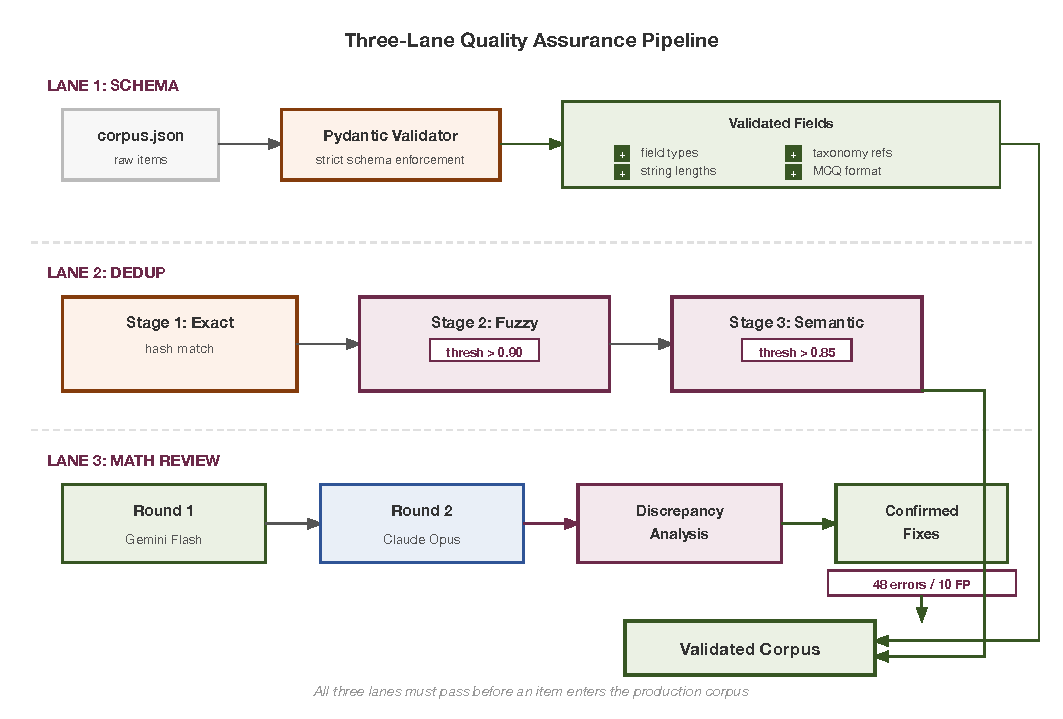
\includegraphics[width=\columnwidth]{fig-quality-pipeline.pdf}
\caption{Multi-stage quality assurance pipeline. Candidate questions pass through schema validation (Pydantic), three-stage deduplication (exact, fuzzy, semantic), and multi-model math verification (Gemini Flash broad review + Claude Opus deep review). Confirmed errors are corrected; duplicates are archived, never deleted.}
\label{fig:quality-pipeline}
\end{figure}

\subsection{Schema Validation}

Every question is validated against a strict Pydantic schema (generated from the LinkML definition) with both field-level and cross-question rules:

\begin{itemize}[nosep]
  \item \textbf{Field constraints}: minimum character lengths (scenario $\geq 50$, napkin\_math $\geq 10$ and must contain a digit), MCQ must have exactly 4 options with correct\_index in $[0,3]$
  \item \textbf{Taxonomy constraints}: topic $\in$ \{79 curated IDs\}, zone $\in$ \{11 ikigai zones\}, track $\in$ \{5 tracks\}, level $\in$ \{L1\ldots L6+\}
  \item \textbf{Uniqueness constraints}: no duplicate IDs, no duplicate (track, title) pairs among published questions
  \item \textbf{Linguistic checks}: no trailing quotes, no markdown formatting artifacts, no placeholder text
\end{itemize}

\subsection{Multi-Stage Deduplication}
\label{sec:dedup}

Following best practices from web-scale deduplication \citep{broder1997minhash} and educational assessment, we employ a three-stage pipeline:

\begin{enumerate}[nosep]
  \item \textbf{Exact match}: Lowercased, whitespace-stripped scenario comparison. Catches copy-paste duplicates.
  \item \textbf{Fuzzy match}: \texttt{difflib.SequenceMatcher} $> 0.90$ within same (track, topic) groups. Catches minor rewordings.
  \item \textbf{Semantic match}: Sentence-BERT cosine similarity $> 0.85$ via ChromaDB. Catches same-concept-different-words duplicates.
\end{enumerate}

Confirmed duplicates are \emph{archived} (status set to ``archived''), never deleted, preserving the audit trail---a practice adopted from Anki's large shared deck management \citep{anking2024}.

\subsection{Multi-Model Math Verification}
\label{sec:math-review}

Napkin math is the soul of \staffml{}---and the most error-prone component. Hardware specifications change across generations, unit conversions cascade, and order-of-magnitude errors are easy to introduce. We verify math through multi-model cross-review:

\begin{enumerate}[nosep]
  \item \textbf{Round 1} (broad): Gemini Flash reviews all questions in 50-question chunks, checking arithmetic, hardware specs, unit consistency, and logical coherence. 63 parallel review jobs complete in $\sim$12 minutes.
  \item \textbf{Round 2} (deep): Claude Opus reviews the same questions independently, catching subtle logical errors that Flash misses.
  \item \textbf{Round 3} (exhaustive): 19 parallel Claude Opus agents, each with track-specific hardware reference sheets, independently recompute \emph{every} calculation from first principles.
  \item \textbf{Discrepancy analysis}: Errors found by one model but not the other are flagged for manual review. False positives are tracked to calibrate reviewer accuracy.
\end{enumerate}

Round 3 uncovered systematic error patterns invisible to earlier passes:

\begin{itemize}[nosep]
  \item \textbf{Multi-factor multiplication truncation} (68 fixes): In TinyML depthwise separable convolution questions, the generation model consistently multiplied only the last two factors in a chain (e.g., $3 \times 3 \times 32 \times 64$ recorded as $512$ instead of $18{,}432$).
  \item \textbf{H100 memory myth} (15 fixes): Multiple questions stated H100 has 40\,GB---likely from early PCIe rumors. All H100 variants ship with 80\,GB HBM3.
  \item \textbf{PCIe bidirectional confusion} (8 fixes): Gen4 x16 provides $\sim$32\,GB/s unidirectional, not 64\,GB/s.
  \item \textbf{KV-cache double-counting} (8 fixes): Several questions included an extra factor of 2, confusing the $K+V$ factor already in the formula with a separate doubling.
\end{itemize}

After three rounds, the confirmed error rate is below 0.05\%.

\subsection{The 19-Check Invariant System}

Beyond per-question validation, \staffml{} enforces \numinvariants{} structural invariants across the three data files (corpus, taxonomy, chains). These checks run as a CI gate---no commit is accepted if any invariant fails:

\begin{enumerate}[nosep]
  \item No duplicate concept names in taxonomy
  \item No duplicate concept IDs in taxonomy
  \item All concept IDs are kebab-case
  \item Question count matches between taxonomy metadata and corpus
  \item Every corpus topic exists in taxonomy
  \item All prerequisite targets exist (no broken edges)
  \item Prerequisite graph is acyclic (DAG check)
  \item All competency areas are canonical (13 valid values)
  \item All levels are canonical (L1--L6+)
  \item No duplicate question IDs in corpus
  \item All chain question IDs exist in corpus
  \item No duplicate (track, title) pairs
  \item No singleton concepts (topics with $<$ 3 questions are flagged)
  \item No corpus-only concepts (topics in questions but not in taxonomy)
  \item Zone coverage: all 11 zones have $\geq 10$ questions
  \item Topic coverage: all 79 topics have $\geq 10$ questions
  \item Topic concentration: no topic has $>$ 10\% of total questions
  \item Chain levels are populated (chains span $\geq 3$ levels)
  \item Validation status consistency (validated flag matches validation fields)
\end{enumerate}

The invariant system catches errors that no single-question validator can detect: a topic that was deleted from the taxonomy but still referenced by 50 questions (check 5), a prerequisite cycle introduced by a new edge (check 7), or a topic that has accumulated an outsized share of questions (check 17).

\subsection{Depth Chain Coherence}
\label{sec:chains}

Depth chains verify that questions on the same topic form a coherent cognitive progression through Bloom's levels. A chain is a sequence of 3--5 questions on the same topic with strictly increasing cognitive demand:

\begin{quote}
\small
L1: ``What is a KV-cache?'' (Remember) \\
$\to$ L3: ``Calculate KV-cache size for Llama-70B'' (Apply) \\
$\to$ L5: ``Server OOM'd at 128K context---diagnose'' (Evaluate) \\
$\to$ L6+: ``Design a PagedAttention allocator'' (Create)
\end{quote}

The corpus currently contains \numchains{} topic clusters spanning 3+ levels, with \numfullchains{} full chains spanning all six levels from L1 to L6+.

% ============================================================================
\section{Coverage Analysis}
\label{sec:coverage}

\subsection{Multi-Axis Coverage}

The primary coverage analysis examines the three-dimensional space of topic $\times$ zone $\times$ track. With \numtopics{} topics, \numzones{} zones, and \numtracks{} tracks, the full space contains $79 \times 11 \times 5 = 4{,}345$ cells. Not all cells are semantically meaningful (e.g., a TinyML question about InfiniBand fabric topology), so coverage targets apply to the subset of valid cells determined by each topic's applicable tracks.

\subsection{Track Distribution}

The current corpus distribution across tracks reflects industry demand:

\begin{table}[h]
\centering
\small
\caption{Question distribution across deployment tracks.}
\label{tab:track-dist}
\begin{tabular}{@{}lrc@{}}
\toprule
\textbf{Track} & \textbf{Questions} & \textbf{Share} \\
\midrule
Cloud & 2{,}845 & 49.2\% \\
Edge & 972 & 16.8\% \\
Mobile & 833 & 14.4\% \\
TinyML & 816 & 14.1\% \\
Global & 320 & 5.5\% \\
\midrule
\textbf{Total} & \textbf{5{,}786} & \textbf{100\%} \\
\bottomrule
\end{tabular}
\end{table}

The cloud track has the densest coverage, reflecting the current industry emphasis on LLM serving and distributed training. TinyML has the sparsest coverage, reflecting the smaller but growing demand for MCU-level ML systems engineering.

\subsection{Zone Distribution}

The zone distribution reveals which cognitive acts are most heavily represented:

\begin{table}[h]
\centering
\small
\caption{Question distribution across ikigai zones.}
\label{tab:zone-dist}
\begin{tabular}{@{}lrc@{}}
\toprule
\textbf{Zone} & \textbf{Questions} & \textbf{Share} \\
\midrule
Diagnosis & 1{,}247 & 21.6\% \\
Recall & 1{,}136 & 19.6\% \\
Evaluation & 990 & 17.1\% \\
Fluency & 913 & 15.8\% \\
Specification & 375 & 6.5\% \\
Design & 366 & 6.3\% \\
Optimization & 323 & 5.6\% \\
Implement & 319 & 5.5\% \\
Mastery & 80 & 1.4\% \\
Realization & 31 & 0.5\% \\
Analyze & 6 & 0.1\% \\
\midrule
\textbf{Total} & \textbf{5{,}786} & \textbf{100\%} \\
\bottomrule
\end{tabular}
\end{table}

Compound zones (diagnosis, evaluation, fluency) dominate the corpus, which is intentional: these are the zones that most sharply differentiate Staff-level candidates. The low counts for pure analyze (6) and realization (31) represent generation targets for the next expansion cycle.

\subsection{Level Distribution}

\begin{table}[h]
\centering
\small
\caption{Level distribution (actual vs.\ target Bloom's pyramid).}
\label{tab:level-dist}
\begin{tabular}{@{}lrrc@{}}
\toprule
\textbf{Level} & \textbf{Questions} & \textbf{Share} & \textbf{Target} \\
\midrule
L1 & 547 & 9.5\% & 17\% \\
L2 & 886 & 15.3\% & 23\% \\
L3 & 1{,}432 & 24.7\% & 23\% \\
L4 & 1{,}258 & 21.7\% & 15\% \\
L5 & 1{,}128 & 19.5\% & 12\% \\
L6+ & 535 & 9.2\% & 10\% \\
\bottomrule
\end{tabular}
\end{table}

The corpus is slightly top-heavy relative to the Bloom's pyramid target: L4--L5 are overrepresented while L1--L2 are underrepresented. This reflects the natural bias of LLM-generated questions toward more complex scenarios. Targeted L1--L2 generation is planned for the next expansion cycle.

% ============================================================================
\section{Infrastructure}
\label{sec:infrastructure}

\subsection{The Vault Toolchain}

All vault operations are consolidated into a CLI toolchain that enforces the methodology described above:

\begin{table}[h]
\centering
\small
\caption{Core vault tools and their methodological role.}
\label{tab:vault-commands}
\begin{tabular}{@{}lll@{}}
\toprule
\textbf{Tool} & \textbf{Role} & \textbf{Method} \\
\midrule
\texttt{schema.py} & Per-question validation & Pydantic / LinkML \\
\texttt{vault\_invariants.py} & Cross-file structural checks & 19 invariants \\
\texttt{scorecard.py} & Coverage dashboard & Topic $\times$ zone $\times$ track \\
\texttt{generate.py} & Question generation & AIG pipeline \\
\texttt{validate\_questions.py} & Math verification & Multi-model \\
\texttt{graph.py} & Taxonomy explorer & Path queries, DOT \\
\texttt{resolve.py} & Topic/zone mapping & Corpus $\to$ taxonomy \\
\texttt{gate.py} & Pipeline gate & Block on regressions \\
\bottomrule
\end{tabular}
\end{table}

\subsection{Generation Pipeline}

Questions are generated using an Automatic Item Generation (AIG) pipeline \citep{gierl2013aig} powered by large language models with multi-agent review. Following Evidence-Centered Design \citep{mislevy2003ecd}, every question begins with a specification of what competency it measures (topic $\times$ zone $\times$ track $\times$ level), what evidence a correct answer would demonstrate (Bloom's cognitive operation), and what task features elicit that evidence (hardware specs, failure mode, scale).

\begin{figure}[t]
\centering
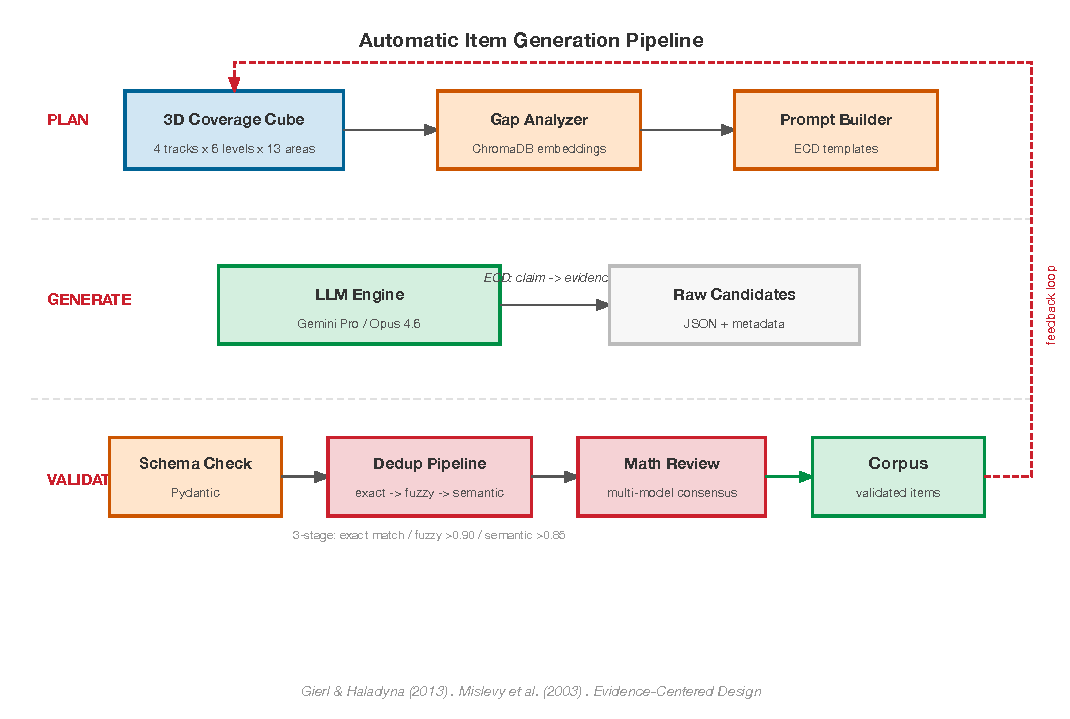
\includegraphics[width=\columnwidth]{fig-generation-pipeline.pdf}
\caption{The Automatic Item Generation pipeline. Gap analysis identifies underfilled cells in the coverage space. Prompts are constructed with hardware constants, Bloom's descriptors, zone descriptions, and track constraints. LLM-generated candidates pass through schema validation, multi-stage deduplication, and multi-model math verification before corpus integration.}
\label{fig:generation-pipeline}
\end{figure}

The generation prompt includes:

\begin{itemize}[nosep]
  \item \textbf{Topic description} from \texttt{taxonomy\_data.yaml}: what concept to test
  \item \textbf{Zone description} from \texttt{zones.py}: how to test it (which skills to exercise)
  \item \textbf{Track constraints}: which physics regime applies
  \item \textbf{Level expectations}: which Bloom's cognitive operation to target
  \item \textbf{Hardware constants} from the \texttt{mlsysim} physics engine (H100: 80\,GB HBM3, 3.35\,TB/s, 989\,TFLOPS FP16; Orin: 275\,TOPS INT8; Cortex-M4: $\sim$100\,MFLOPS, 256\,KB SRAM)
\end{itemize}

The four-axis classification is specified \emph{before} generation, ensuring coverage is intentional rather than emergent. Gap analysis identifies underfilled cells in the topic $\times$ zone $\times$ track space; the generation engine targets those cells explicitly.

\subsection{Data Architecture}

The vault consists of three core data files, each serving a distinct role:

\begin{itemize}[nosep]
  \item \textbf{\texttt{corpus.json}} (\numquestions{} questions): Every question carries \texttt{topic}, \texttt{zone}, \texttt{track}, and \texttt{level} fields validated against the schema. Legacy fields (\texttt{primary\_concept}, \texttt{reasoning\_mode}) are retained for backward compatibility but are not maintained.
  \item \textbf{\texttt{taxonomy\_data.yaml}} (\numtopics{} topics, \numedges{} edges): The curated knowledge graph, defined in YAML and validated against the LinkML schema.
  \item \textbf{\texttt{chains.json}} (\numchains{} chains): Depth chains linking questions on the same topic across Bloom's levels.
\end{itemize}

\subsection{Mastery Levels and Bloom's Mapping}

Six mastery levels map directly to Bloom's revised taxonomy \citep{anderson2001taxonomy} and industry engineering ladders:

\begin{table}[h]
\centering
\small
\caption{Mastery levels mapped to Bloom's taxonomy and industry ladders.}
\label{tab:levels}
\begin{tabular}{@{}llll@{}}
\toprule
\textbf{Level} & \textbf{Bloom's} & \textbf{Scope} & \textbf{Industry} \\
\midrule
L1 & Remember & Own a task & Intern \\
L2 & Understand & Own a task & Intern \\
L3 & Apply & Own a task & New Grad \\
L4 & Analyze & Own a component & Mid (L4) \\
L5 & Evaluate & Own a system & Senior (L5) \\
L6+ & Create & Own architecture & Staff+ (L6) \\
\bottomrule
\end{tabular}
\end{table}

Each level tests a qualitatively different cognitive operation. L1 requires memorization of physical constants (``HBM3 latency is $\sim$300\,ns''). L3 requires applying a formula to a novel scenario (``Calculate KV-cache size for Llama-70B at 128K context''). L6+ requires synthesizing novel architectures from first principles (``Design a scheduling policy that prevents prefill starvation under continuous batching'').

% ============================================================================
\section{Status and Future Work}
\label{sec:status}

As of \today, the \staffml{} vault contains \numquestions{} questions with four-axis classification (topic, zone, track, level) enforced by the LinkML-generated schema and \numinvariants{} structural invariants.

\textbf{Completed milestones}:
\begin{itemize}[nosep]
  \item \textbf{Ikigai competency model}: 4 skills, 11 zones, deployed across all \numquestions{} questions.
  \item \textbf{Topic taxonomy}: \numtopics{} curated topics across \numareas{} competency areas with \numedges{} typed prerequisite/related edges. Schema defined in LinkML.
  \item \textbf{Math verification}: Three rounds of multi-model verification. Confirmed error rate $< 0.05\%$.
  \item \textbf{Invariant system}: \numinvariants{} automated cross-file checks running as CI gate.
  \item \textbf{Depth chains}: \numchains{} chains built (\numfullchains{} spanning all 6 levels L1$\to$L6+).
  \item \textbf{Schema validation}: All \numquestions{} questions pass Pydantic validation. Zero errors.
  \item \textbf{Deduplication}: 3-stage pipeline operational. Zero exact duplicates in current corpus.
\end{itemize}

\textbf{Planned work}:
\begin{enumerate}[nosep]
  \item Fill zone gaps: generate realization (31 questions) and pure analyze (6 questions) to minimum threshold of 100 each
  \item Fill level gaps: generate L1/L2 questions to reach Bloom's pyramid target distribution
  \item Cross-track expansion: generate edge/mobile/TinyML variants for cloud-heavy topics
  \item IRT calibration from user interaction data ($\geq 30$ responses per item) \citep{lord1980irt}
  \item Community contribution pipeline with automated validation
  \item Adaptive question selection based on user performance profiles across zones
  \item Taxonomy refresh cycle (6-month cadence per inclusion framework)
  \item Graph-guided study paths: use the prerequisite graph to generate personalized topic sequences
  \item QTI export for LMS integration \citep{qti2020}
\end{enumerate}

% ============================================================================
\bibliography{references}

\end{document}
